\documentclass[a4paper, twocolumn]{article}

\usepackage[english]{babel}
\usepackage[utf8]{inputenc}
\usepackage{amsmath}
\usepackage{graphicx}
\usepackage[colorinlistoftodos]{todonotes}

%added by vipandey
\usepackage{multirow}
\usepackage{hyperref}
\usepackage{placeins}
%\usepackage{float}
%\restylefloat{table}

\usepackage{titling}
\newcommand{\subtitle}[1]{%
 \posttitle{%
 \par\end{center}
 \begin{center}\large#1\end{center}
 \vskip0.5em}%
}

\usepackage{comment}

%\usepackage{tabularx}

%\usepackage[showframe]{geometry}% http://ctan.org/pkg/geometry
%\usepackage{lipsum}% http://ctan.org/pkg/lipsum
%\usepackage{multicol}% http://ctan.org/pkg/multicols
%\usepackage{graphicx}% http://ctan.org/pkg/graphicx


\title{“But does it scale?”: \\Verifying the heuristics of scaling a web application}
\subtitle{Project submission towards CSE 223B - Spring 2014}

\author{K Sree Harsha, Amirsaman Memaripour, Vineet Pandey}

\date{\today}

\begin{document}
\maketitle

\begin{abstract}
Web applications drive the internet economy. With millions of users and a variety of services, these applications bring forth interesting scalability challenges hitherto unseen for distributed applications. Efforts to extract optimum performance from available resources has lead to tweaks at all levels of the software stack inclusing application, network, filesystem and storage. When a single node does not meet the performance requirements, the load is distributed across multiple backends which need to intelligently manage the control and data without introducing new problems. In our study, we intend to verify the known heuristics for scaling a web application. We examine an IM application - a representative of the modern million-user web application and start from a stock build to optimize its performance. We tweak the software and system configuration and use both scale up and scale out methods to extract high performance. In our results, we managed to scale an open-source  XMPP server on a typical desktop hardware configuration to support more than 80K messages per second in a high-stress environment. In the process, we learnt important lessons about profiling a software and finding bottlenecks at multiple levels - application code, system environment and hardware. 
\end{abstract}

\section{Introduction}
Web applications drive the internet economy and demand scalability challenges hitherto unknown with normal applications. Applications such as Facebook, WhatsApp and Twitter are examples of server applications which do most of their computation on the server and transfer the data to client for suitable layout. Though lack of network connection is much less prevelant now than 20 years ago, modern browsers and mobile apps are capable of caching a large amount of data and perform some procesing even when offline. However, we expect most services to continue running in a centralized way for technical and business reasons and believe that optimizing the performance on the server side will continue to be relevant for the foreseeable future. 

We present statistics for popular IM service WhatsApp~\cite{w1} which show the current requirements of web scale applications. Whatsapp handles 320 million daily users~\cite{w2}, handles 19 billion daily sent messages and 34 billion daily received messages with a peak count of 64 billion received messages (the difference between sent and received messages is due to muticasts)~\cite{w3} . Assuming 32B messages, it averages to ~400K messages/sec, while WhatsApp has mentioned that they service can handle up to 2M messages/sec. 

In our project, we intend to verify some known scalability techniques which allow an IM application to provide high-quality service to users. We primarily consider server side optimizations (though our client also went through iterative improvements) and we use multiple technologies to test and monitor our system to draw broader insights. In our report, we have also explained the rationale behind our decisions, while prototyping, profiling and finding bottlenecks.

We chose this topic because of multiple factors: 
\begin{enumerate}
\item We intend to find the challenges in building a web service similar to the ones we regularly use. 
\item We intended to use the credits for EC2 platform. This gave us ideas about large-scale test of software since we would not have to bother about setting up a lot of systems and ensuring that their health is fine. 
\item Coming from a systems background, we want to learn hacks about optimizing the backend to better understand interaction between an application, system software and hardware. 
\end{enumerate}

\noindent Our chief contributions from the project include scaling Openfire XMPP server by fixing memory issues, scaling single-node ejabberd by fixing multiple bottlenecks across the stack and enabling logging client messages to a NoSQL database. 

Through the project, our objective was to poke around at various factors which causes bottlenecks in our system's performance. We have also shared our experience working and firefighting with EC2 platform and we believe such experience-driven learning will help other systems builders as much as they will help us in rapid prototyping and performance optimization. 

\section{Service description}
We build an instant messaging application using available open source technologies and measure its performance. 

\subsection{Service workflow}
Assume two users Alice and Bob who will communicate over Instant messaging. 
\begin{enumerate}
\item Alice creates an account with the server 
\item Alice logs in to the server
\item Alice adds Bob as a friend (accepted by default)
\item Alice sends message to Bob
\item Bob reads messages and replies
\end{enumerate}
Steps 4 anf 5 repeat and form the major source of load on the server when the number of user and messages scales up. In further sections, we build upon this idea to stress-test our system. 

\subsection{Unsupported features}
We provide basic one-to-one instant messaging capability to the users. We do not support sharing files or group messaging. We believe a basic version of these services can be simulated by our system (for example, sending MB-sized messages to simulate images) and we did not have the time to design and test an optimized system for these workloads. 

Our client is a terminal utility and we did not build a GUI for it, since it does not affect the core facilities provided by us. Our messages are of uniform size 128 bytes to make it similar in size to the popular 140 character message limit (on SMS and Twitter). 

\subsection{Different modes of operation}
Our instant messaging client works in different modes.

\begin{enumerate}
\item \textbf{YOLO mode}: In this mode, the client does not store any data with the server. All messages sent by Alice are immediately forwarded by Bob to the server, and the server does not store a copy. This is similar to how WhatsApp works. 

\item \textbf{Forever mode}: The client stores all its messages with the server. Furthermore, the server does not require the client’s password to access its previous logs, and it can read or run data analytics on the chat logs at any suitable time. We believe this is similar to how Facebook chat works. 
\end{enumerate}
We have tried optimizing separately for these modes in our work. 


\section{Implementation details}
\subsection{XMPP}
Our clients and servers use XMPP~\cite{xmpp} as the underlying messaging protocol. Popularized by Jabber, XMPP forms the backbone of most popular IM service including Google Talk, WhatsApp and Facebook Chat. XMPP works with messages in XML format and the XMPP library provides support (such as encapsulation/decapsulation primitives) for implementing one's own service on top. 

\subsection{Client}
The client side is a minimal implementation of an XMPP client using Smack library~\cite{smack}, which is a free Java library from Ignite Realtime. By default, Smack provides connection objects that can be used to connect to the XMPP server.  Additionally, Smack provides a set of classes that can be used to register for incoming messages, including status updates and chat messages. Using this library, the client side does not need to engage in low-level transmission logic of a chat client and can focus on user-related activities such as receiving message content and displaying user-driven notifications.

We went through multiple iteratins of improving the client, some of which are described below. 
\begin{enumerate}
\item \textbf{First implementation}: We built a minimal XMPP client without any embedded test-logic since our focus was on sending throguh as much data as possible on server to stress the server and we did not concern ourselves with client-side efficiency.

\item \textbf{Issues with the first implementation}: We found that smack library would start too many Java VMs on a client machine to simulate realistic workload and also use up more open ports than the system could provide. We also ran into synchronizing issues with the clients.

\item \textbf{Synchronizing the clients}: We used a basic approach by overloading the definition of a file to act like a shared lock: all clients wait in a loop till the time that a file created by the parent process disappears. The parent process is a bash script that basically creates all VMs and waits for their completion. We used an estimate for the time taken by the clients to successfully connect to the server, so that we can delete the shared lock and signal them to continue. 

\item \textbf{Synchronizing clients across machines}: In the basic implementation, clients need to have the target in their contact list to be able to send messages, thus they need to wait to have all their contacts online! In order to solve this problem, we removed all inter-node communications that requires synchronization between all client machines. This problem is inherently difficult to solve since we are using machines with different hardware configurations and network delays which had different processing times. For example, by the time our EC2 VM client sent out its first message, our local desktop had already finished with sending all the messages! In the new scheme, each client only communicates with other clients on the same physical machine.

\item \textbf{Java machine per client}: We faced another issue which originates from the fact that we needed to create a new Java virtual machine per client. This simply requires having too many powerful systems for running clients, which is not feasible in our case. In order to tackle this problem, we created a new program that basically simulates the behavior of multiple clients on a single Java virtual machine. All the parameters, including the number of clients that it should imitate and the number of messages that each client should send out are configurable. Moreover, the new client does not need to have the message target in its contact list and can freely send messages to any other client in the system. This allows us to scale the number of clients to any arbitrary number.
\end{enumerate}

\subsection{Yolo mode}
In Yolo mode, the messages are not stored by the server. During development and testing, we automatically added all $1600$ users to the server by scripting it rather than waiting for every user to create its own account at message sending time since that would throttle our message rate. We configered our server to not store any incoming messages and instantly forward the messages to the receving client. However, the results indicate that the server software still reads the message into the buffer and then sends it out, which would be an extra buffer swap. We considered this a potential low-level optimization for future work.  

\subsection{Forever mode}
In Forever mode, the server stores the messages and hence, we need to make decisions about the technologies to use for the same. We used the vanilla database provided by our stock server but later moved to MySQL and MongoDB to optimize on client accesses, especially in a clustered setting. 

\subsection{Openfire}
Openfire is an instant messaging (IM) and groupchat server implemented in Java which uses XMPP. It claims to support support more than 50,000 concurrent users; however, this depends on the message distribution. Openfire provides an easy to use web console which helps novice admins and it is widely deployed as a mid-range business IM solution. The code has support for multiple features with good documentation and the server also allows extensibility using plugins. The software has good online support.  

Openfire's XMPP server implementation has two main architectural choices:
\begin{enumerate}
\item \textbf{Pubsub model}~\cite{pubsub}: Publish–subscribe is a messaging pattern where senders of messages, called publishers, do not program the messages to be sent directly to specific receivers, called subscribers. Instead, published messages are characterized into classes, without knowledge of specific subscribers, if any. Similarly, subscribers express interest in one or more classes, and only receive messages that are of interest, without knowing about publishers. This layer of indirection allows for flexible transfer of messages. 

\item \textbf{BOSH}: Bidirectional-streams Over Synchronous HTTP (BOSH)~\cite{bosh} is a transport protocol that emulates a bidirectional stream between two entities (such as a client and a server) by using multiple synchronous HTTP request/response pairs without requiring the use of polling or asynchronous chunking. XMPP over BOSH is the popular implementation for IM servers supprting traffic over web. 
\end{enumerate}
For some of our experiments, we enabled logging and clustering in Openfire. 
\begin{itemize}
\item \textbf{Logging using Mongodb}:
Openfire server can log messages (chats) using a plugin called monitoring~\cite{plugin_monitoring}. However, Openfire currently supports only SQL databases, hence we modified  the monitoring plugin to log  all the messages in MongoDB~\cite{mongodb} instead of SQL database since our objective is to provide access to a MongoDB server for a cluster of openfire servers. We believe MongoDB is a wiser choice than SQL databases because of the relaxed consistency semantics which yields better performance when messages arrive at a high ingest rate (as in our workload). SQL databses provide strict consistency which is not necessary for our case since there is hardly any write-contention for a written element. As the number of messages scales up, we expect SQL databases to become a bottleneck. 

We created a new db connection for the MongoDB database and used this connection in the plugin to save the records to MongoDB and modified the compilation of Openfire to build it with the MongoDB jar. 

\item \textbf{Clustering Openfire}: For clustering using openfire, we used  a plugin called Hazelcast~\cite{hazelcast} which allows clustering multiple instances of the servers. We scaled the number of instances as a power of two to allow the software to do symmetric partitioning of associated tasks. We faced minor issues in resolving the private IP configuration presented by Amazon EC2. 
\end{itemize}

%\newpage
\subsection{ejabberd}
Most of our optimizations concern ejabberd, an XMPP server which leverages Erlang's advantages to provide a high-throughput fault-tolerant cluster-ready server. ejabberd has become the server of choice for most web IM services serving millions of users, including WhatsApp and Facebook Chat. Though the IM servers have optimized stock ejabberd further, the code is not publicly available and we started our experiments with stock ejabberd code and modifying its environment to yield better performance.

ejabberd also supports a PubSub model and IRC transport but rather than using a light version of SQL databse (like Openfire), ejabberd has its own NoSQL database mnesia~\cite{mnesia} which is used to maintain configuration and state information in tables~\cite{ej1}. mnesia database can be kept in different modes: ramonly,disconly or ram and disc. For a clustered server, mnesia provides the option to decide which tables to share between the nodes using table\_copy primitives. The configuration can be adjusted by extra modules to log message data to the mnesia database as well. 

Built on top of Erlang~\cite{erlang}, ejabberd has a flexible structure where modules can be inserted and removed from the codebase. Erlang provides extremely lightweight processes (easily running 30K erl processes on its VM) and actor model (explicit message passing) making it (conceptually) easier to debug. It also allows for hot code-swapping which allows the administrator to replace a module in a running ejabberd instance without doing a stop-the-world upgrade. Typical benchmark results put ejabberd's throughout at 2K messages/second on a 1.5 GHz machine, however, WhatsApp has successfully scaled a 32-core mchine to run ejabberd which can handle 2M connections per second. In our project, we were able to successfully go above 80K connections per second with a 4-core machine and lesser RAM. Since ejabberd runs in the Erlang VM, it provides cross-platform operation which is an added advantage since the application does not need to be highly system dependent. 

However, despite these massive advantages, ejabberd lacks in documentation and the Erlang codebase and configuration requires a steep learning curve which make it challenging to begin working with. 

\textbf{Clustering: }
We ran a cluster of ejabberd nodes to see the performance scaling and resource utilization across different nodes. The clustering is straightforward but demands a good understanding of various mensia tables to ensure that redundant copies of some tables are not created which might affect the performance. 

We have described our workload in detail in the Performance section. 

\section{Previous work and scaling heuristics}

The domain of Instant messaging applications has been rich with success stories since the internet boom. Early messaging software like IRC and contemporary ones like Hangouts (formerly Google Talk), Facebook Chat and WhatsApp have used different techniques to provide the same basic functionality to the users of being able to send and receive messages in real time. We closely followed WhatsApp infrastructure~\cite{w4} from public sources and it helped us in a number of our decisions and discussions in later sections of the paper. 

While looking at Instant messaging software, we also looked at other web applications to find out about typical scaling problems and steps taken to solve those. We studied Instagram, Twitter and Youtube~\cite{instagram_ppt,youtube,twitter} to avoid their scalability issues and draw ideas about how to solve the issues we faced. A summary of our heuristics study is mentioned in Table~\ref{tab:heuristics} and the categories are mentioned in Table~\ref{tab:categories}. 

It is difficult to describe all the heuristics in detail but between Openfire and ejabberd, the latter seemed to meet many of the criteria as mentioned in its descrption. ejabberd creates light-weight processes, has a modular structure and allows easy DB factoring with mnesia. 

%\FloatBarrier
\begin{table}
\centering
\begin{tabular}{|l|l|}
\hline
\bf{Label} & \bf{Category} \\
\hline
Cap & Capacity \\
Avl & Availability \\
Dev & Development Effort \\
Perf & Performance (client latency + \\
& system throughput)\\
\hline
\end{tabular}
\caption{\label{tab:categories}Categories relevant for building a scalable web application}
\end{table}
%\FloatBarrier

\FloatBarrier
\begin{table*}
\centering
\begin{tabular}{|l|l|l|}
\hline
{\bf{Sl.}} & \multirow{2}{*}{\bf{Technique}} & \multirow{2}{*}{\bf{Categories}} \\
\bf{num} & & \\
\hline
1 & Maximize connections on a server & Cap,Perf \\
2 & Avoid using locks & Perf \\
\multirow{2}{*}{3} & Outsource extreme cases & \multirow{2}{*}{Perf} \\
& (like youtube popular videos to a CDN) & \\
4 & Use stateless backends & Dev,Perf \\
5 & DB scaling: Partition then factor & Dev,Perf\\
\multirow{2}{*}{6} & Application code structure & \multirow{2}{*}{Dev,Perf} \\
& and choice of language - modular, APIs & \\
7 & Smart caching & Perf\\
8 & Profiling and modifying stack accordingly & Perf\\
9 & Replication strategy - trade-offs & Avl\\
\hline
\end{tabular}
\caption{\label{tab:heuristics}Heuristics used by web applications to improve scalability}
\end{table*}
%\FloatBarrier



\section{Experiment setup}

\subsection{Infrastructure \& testbed}

Table~\ref{tab:machine} shows the options available to us on EC2 infrastructure for machines~\cite{ec2_1}. 

\FloatBarrier
\begin{table*}
\centering
\begin{tabular}{|l|l|l|l|l|l|l|}
\hline
\bf{Instance type} & \bf{vCPU*} & \bf{Memory} & \bf{Storage} & \bf{Networking} & \bf{Physical processor} & \bf{Clock} \\
&&(GB)&(GB)&&&\bf{(GHz)}\\
\hline
t1.micro & 1 & 0.613 & EBS Only & Very Low & Variable & - \\
m3.medium & 1 & 3.75 & 1 x 4 SSD & Moderate & Intel Xeon E5-2670 v2 & 2.5\\
m3.large & 2 & 7.5 & 1 x 32 SSD & Moderate & Intel Xeon E5-2670 v2 & 2.5\\
m3.xlarge & 4 & 15 & 2 x 40 SSD & Moderate & Intel Xeon E5-2670 v2* & 2.5 \\
c3.8xlarge** & 32 & 60 & 2 x 320 SSD & 10 Gigabit & Intel Xeon E5-2680 v2 & 2.8\\
\hline
\end{tabular}
\caption{\label{tab:machine}Machine options on EC2}
\noindent *A vCPU is ``One EC2 Compute Unit provides the equivalent CPU capacity of a 1.0-1.2 GHz 2007 Opteron or 2007 Xeon processor. This is also the equivalent to an early-2006 1.7 GHz Xeon processor"~\cite{ec2_1}.\\
** We wanted to use this instance because the WhatsApp server which managed 2Million connections per server had a similar configuration (32 cores). 
\end{table*}

\subsection{Software servers}
We had multiple open source servers to choose from to build our solution. We list these options in Table~\ref{tab:servers} and provide a brief analysis of the rationale behind our choice. 

\begin{table*}
\centering
\begin{tabular}{|l|l|l|l|l|}
\hline
\bf{Server} & \bf{Assumed} & \bf{Community} & \bf{Implementation} & \bf{Ease of}\\
& \bf{Performance}& \bf{support}& \bf{Language}&  \bf{working}\\
\hline
jabberd & Med & Med & C/C++ & Low\\
jabberd 2.x & Med & Med & C & High\\
Openfire & Med & High & Java & High\\
ejabberd & High & Low & Erlang & Low\\
\hline
\end{tabular}
\caption{\label{tab:servers}Comparison for different server options}
\end{table*}

Both jabberd and jabberd 2.x are implemented in C/C++ and hence, are expected to perform better than Java-based Openfire. However, due to the concurrent nature of task, ejabberd's performance is expected to be much better due to light-weight processes. However, ejabberd has poor community support compared to Openfire. Since jabberd* are not popular anymore, it is more difficult to get answers for those stacks. 

An interesting point for us was the programming language used to implement the server. While C is efficient, it would require much more effort and we could spend our time doing more things in high level languages. Hence, we wanted to choose between Openfire and ejabberd and finally decided to test both for our workloads. In terms of perceived ease of working, we believed Java-based Openfire would definitely be easier than ejabberd. For our small benchmarking effort, we did not pay much attention to factors such as compliance to the xmpp standards (xep- rfcs) or support of advanced features. 


\subsection{Load Balancing}
We used load balancers to distribute the load across multiple servers when working in clustered mode. We used Amazon Elastic Load Balancing (ELB)~\cite{ec2_2} for its ease of use since all our server instances run on EC2. We considered using HAProxy due to more favourable reviews online but persisted with ELB since it seemed to work well enough for our requirements. ELB provides a public IP address which can be contacted by clients while it internally acceses the servers to distribute the load. 

\subsection{Client-side efficiency}
We have covered these issues in our description of client in Section 3.2

\subsection{Workload}
In order to measure the performance of each setup, we needed to either build an application that imitates users behavior or employ available benchmarking tools. Although there are some XMPP benchmarking tools, we prefered to develop our own workload generator to have more control over different parameters that can affect the functionality of our server. For instance, you have the option to change the time between each message, size of each message, number of clients and the number of contacts each client send messages in our client program.

In our experiments, we used 1600 users each sending 500 messages to 10 contacts, leading to a total number of 8 million messages. Each message is 128 bytes, which is close to the average size of text messages exchanged through Internet messaging services.
	
    
\subsection{Measurement tools}
Throughout our experiemnts, we wrote scripts to monitor the resource utilization on client and server machines. These can be found on github at \url{https://github.com/samanca/whatsup}. Our scripts based on vmstat, iostat etc. 


We also used many freely available and priced tools to monitor the graphs of our 20 client machines and servers (depending on cluster configuration). We have mentioned most of them in Table~\ref{tab:tools_mon}. 

\FloatBarrier
\begin{table*}[b]
\centering
\begin{tabular}{|l|l|l|l|}
\hline
\bf{Name} & \bf{Measured quantity} & \bf{Granularity} & \bf{Cost}\\
\hline
Munin~\cite{tools_munin}& Network&1 min & Free\\
\hline
Amazon Cloud Monitoring~\cite{tools_amazonc}& Network CPU Memory Disk & 1 min & Free\\
\hline
Amazon Detailed Monitoring~\cite{tools_amazond}& Network CPU Memory Disk& 30 seconds & Cheap\\
\hline
\multirow{3}{*}{CopperEgg~\cite{tools_copper}}& {Network} & \multirow{3}{*}{1 second} & \multirow{3}{*}{Free}\\
& CPU & & \\
& Memory & & \\
\hline
\end{tabular}
\caption{\label{tab:tools_mon}Different tools used to monitor resources}
\end{table*}


We used CopperEgg to locate problems in our client or server machines (for example, traffic shaping problem). The other tools were not useful due to their coarse granularity of measurements - 1 minute. We did a rough check of the overhead of measurement and found that the services had negligible effect on the running time of the system since they used little resources. 

\subsection{Scaling the message logging database}

We used MongoDB to log all the chat messages exchanged between clients.MongoDB is a cross-platform, document oriented database that provides, high performance, high availability, and easy scalability. 



%\newpage
\section{Performance}
\subsection{openfire}
\subsubsection{Single node}
When we ran experiments for one node and found  ejabber was comprehesively better than openfire interms of messages ,user supported and interms of resource utilization.Detailed graphs are provided in appendix section.

\subsubsection{Cluster}
We realized on one node does not provide good performance , so we scaled out openfire for multiple nodes. We ran our experiments for openfire on cluster sizes 2,4 and 8 and observed the performance.The results of all experiment are in appendix however, performance of clustered openfire as still inferior to ejabberd on one node after our optimization.

\subsubsection{Logging}

As shown in reference section logging was taking more time than non logging.We also observed long tail effect , most of client request would finish less than half the total time however there would be few client requests which would take more time ,this is due to contention of resources after server has already recieved large number of messages. For further details of loggin performance please refer to appendix.

\subsection{ejabberd}
\subsubsection{Single node}
In all our tests across all machines ejabbered performed better than openfire even when we ran openfire on better hardward machine , ejabberd could still accept more messages without crashing. The detailed graphs are in appendix.
\subsubsection{Cluster}
Since the performance of ejabberd on one node was better we scaled ejabberd to 2 nodes and observed.
results can be found in appendix section.



%\begin{table*}[b]
%\centering
%\begin{tabular}{|l|l|l|l|l|}
%\hline
%\bf{Server} & \bf{Assumed performance} & \bf{Number of users} & \bf{Number of messages} & \bf{time taken} \\
%\hline

%\end{tabular}
%\caption{\label{tab:comparison_server}Comparative performance of Openfire and ejabberd }
%//\end{table*}

Having same hardware specification for Openfire and ejabberd, we have been observing quite different performance results for these two in terms of number of messages per second and also memory and processor utilization. One of the main differences here stems from the fact that ejabberd is implemented using Erlang, which is a language inherently designed for concurrent applications and services with high-levels of concurrency. On the other hand, Openfire is implemented in Java, which makes it easy to maintain but hard to scale.

In case of resource utilization, both can take advantage of available hardware resources, e.g. memory and processor, by having a well tuned configuration file. However, ejabberd can provide better throughput in terms of number of messages per second while using exactly same hardware configuration with Openfire. In some experiments, we reached better performance by a factor of 10 with ejabberd compared to Openfire. In the Appendix sectoin, we have some graphs that can provide better understanding about the difference between the throughput of ejabberd and Openfire.

\subsection{ejabberd profiling}
We used eprof~\cite{erl_eprof} and fprof~\cite{erl_fprof} profiling tools. Table~\ref{tab:profiling} presents a comparison of the two approaches. 

\FloatBarrier
\begin{table*}
\centering
\begin{tabular}{|l|l|l|}
\hline
\textbf{Factors/Profiling technique} & \bf{eprof} & \bf{fprof}\\
\hline
\multirow{2}{*} {Execution strategy} & Uses built-in tracing support  & Creates a trace of the entire program \\
&for specific functions at run-time & to be analyzed after program execution \\
\hline
\multirow{2}{*}{Recompilation needed?} & Yes, after adding eprof  & \multirow{2}{*}{No} \\
& functions at relevant functions & \\
\hline
Effect on program & \multirow{2}{*}{High} & \multirow{2}{*}{Low} \\
execution time? & & \\
\hline
\multirow{2}{*}{Specificity} & \multirow{2}{*}{Can select functions} &  Functions in all \\
& & loaded modules \\
\hline
\end{tabular}
\caption{\label{tab:profiling}Profiling tools with ejabberd}
\end{table*}

Since we intend to measure the overall performance of the stock ejabberd program, fprof is a good tool to get the first-cut value for the performance of different modules in ejabberd. Furthermore, ejabberd provides a profiling library $p1_prof$ built on top of eprof and fprof which we have used. 

Unfortunately, running $p1_prof$ with fprof on the server while running our experiments would crash our system since the trace file being generated was too large (4GB+) for the length of the experiment.

%\subsection{Development cost and testing}
%//A graph for results obtained versus time spent (in days)

\section{Optimizations and effect}
\begin{table*}
\centering
\begin{tabular}{|l|l|l|l|l|}
\hline
& \bf{System:} & \bf{System:} & \bf{Software:}  & \bf{Software:}\\
& \bf{kernel} &\bf{user}& \bf{Parameters}& \bf{RTE}\\
\hline
\multirow{3}{*}{CPU} & Max num of processes & & & No. of erlang  \\
&Kernel polling: \tt{+K, epoll}& - & - & processes: \tt{+P} \\
&Async threads&  &  &Pool: \tt{+A}  \\
\hline
\multirow{2}{*}{Memory} & Number of filehandles  & Number of filehandles & \underline{\tt{max\_fsm\_queue}} & \underline{\tt{-Xms$\langle$ size$\rangle$}}\\
&\tt{fs.max-size}&\underline{\tt{(ulimit -n)}}& &\\
\hline
\multirow{3}{*}{Network} &  & Network Queue size &  &  \\
&{\tt{sysctl}} & \tt{TCP\_KEEPALIVE}  & \underline{Shaper value} &\tt{ERL\_MAX\_PORTS} \\
&optimizations & \tt{/proc/sys/net/} & & \tt{ERL\_MAX\_ETS\_TABLES} \\
& & \tt{ipv4/tcp\_tw\_reuse}& & \\
\hline
\end{tabular}
\caption{\label{tab:opt}Single node optimizations to scale up ejabberd. Values modified by us are shown underlined while the system variable names are shown in \texttt{typewriter} font. RTE = RunTime Environment}
\end{table*}

Table~\ref{tab:opt} shows the optimizations performed. We have divided the optimizations according to the resource optimized as and whether the optimization changed the system settings, the software configuration or the software runtime. Please note that we did not do any optimization for disks for our runs since we consistency hit bottlenecks with system settings and memory itself. A brief description is presented here. 
\begin{itemize}
\item Max num of processes: If the application starts too many processes on the system, then it could run out of processes leading to undefined behaviour. Since both our servers run on their own Virual Machines, we did not face these issues at the system level. 
\item Kernel polling: Can siginificantly improve performance when dealing with large number of file descriptors 
\item Async threads: provides better performance than blocking calls. 
\item Number of filehandles: This was the first bottleneck that we hit. ejabberd would run out of filehandles for incoming messages and crash. We increased this limit using \texttt{ulimit -n}. Interestingly, this was the exct first problem faced by Instagram~\cite{instagram_ppt} when they hit the ``Slashdot effect"~\cite{slashdot}. 
\item \texttt{max\_fsm\_queue}: This option specifies the maximum number of elements in the queue of the FSM (Finite State Machine) in ejabberd and increasing this value (if the system can sustan it) can lead to performance improvement if empty queues are the problem. 
\item Network optimizations: Keep TCP alive for a longer duration to avoid the cost of connection teardown and reset, increase the network queue size and reuse the current buffers. However, we did not end up changing these settings~\cite{network_tuning} since network buffer issues did not show up for our servers. 
\item Traffic shaping: this was a major source of pain since the servers were shaping the network according to their pre-configured values. We changed the profile of incoming packets to fully saturate the server, else the client would stop sending messages due to backpressure from server. 
\item \texttt{erl +A +P}: \texttt{+A} flag changes the size of pool from which Erlang Virtual Machine (Beam) chooses the processes. Similarly \texttt{+P} changes the maximum number of erlang processes. In general, we found Beam to be highly efficient and it did not consume all the processor/memory on our systems. 
\item \texttt{ERL\_MAX\_PORTS} \texttt{ERL\_MAX\_ETS\_TABLES}: allow changing the maximum number of ports and tables for the Erlang VM. We did not need to change these settings. 
\end{itemize}

\subsection{Case study: traffic shaping}
We faced difficulty with the traffic shaping because of our unawareness. Early on in our tests, we noticed a problem where the clients would send messages to ejabberd server at 90\%+ CPU utilization and would then drop to very low values. This caused the test to linger for a long time and did not provide correct results since the server wasn't stressed. While debugging this issues, we made a number of checks, such as the heap size on client side (since Smack is written in Java which can be memory intensive) and on the server side (in case the server reached peak memory utilization and just dropped all packets and sent backpressure to clients). We even tried different JRE (Openjdk,SunJDK) to check if we had hit some surprising bug. However, none of these were the issues and we found that there are ``shaper" configurations in ejabberd which define the maximum rates at which the server can accept incoming messages or send outgoing messages. The value was set to 50K/sec which was small for our tests. Increasing this value fixed our issue. 

\subsection{Further scope for optimizations}
We did not implement many optimizations mentioned in the above table. We also found further ways to tune the performance but skipped them for lack of time. Some of them include
\begin{itemize}
\item \textbf{Sweet spot for memory usage}: Since incoming data, outgoing data, network queues, configuration structure and all related data and control structures occupy memory, we think it would be interesting to do some memory profiling to understand which structures take most memory and how to distribute memory among competing needs (network vs filesystem) for optimum performance. This could potentially allow high level of performance at reduced memory requirements. 
\item \textbf{Reusing ports}: by toggling \texttt{SO\_REUSEPORT}.
\item \textbf{Effect of removing modules}: We could potentially strip down our servers to include just the modules needed for their functioning. This would be easier in ejabberd because of it's modular structure while it might require more careful understanding of codeflow and interactions between different components in Openfire
\item \textbf{Heterogenous cluster configuration}: We ran our clustered setup on identical EC2 instances and did not look into using a more heterogenous machine profile to allow for other setups, for example: master-slave configuration.
\item \textbf{Optimizing network queue}: We did not consider working with the system's queuing strategy or the queue sizes. 
\item \textbf{TCP Stack errors}: We noticed errors on TCP stack about failure of some packets but did not fix them or optimize for them since the protocol would take care of it.  Reducing these errors could potentially lead to better network usage but network wasn't a bottleneck for us. 
\end{itemize}


\section{Problems faced}
We faced a number of issues while working on the project and we have listed them here for the community to be aware of them. 

\subsection{EC2 problems}
Since we were using EC2 infrastructure for the first time, a number of our initial issues came from not knowing about the limitations of the platform. For example, EC2 places a limit on the number of machines one user could keep turned on at any given instant (it was 20 for us). We submitted a request to increase this limit but we did not hear from the support team. Similarly, we had to provide a special request to use a compute-intensive machine which became available to us after 2 business days (over a weekend!). We had to structure our experiments to ensure that we did not breach the limits improsed by EC2 on how many machines of a certain insance we could use. Similarly, static IPs (called Elastic IPs on EC2~\cite{ec2_3})  are a scarce resource (5 per user) and we had to use them suitably. 

We tried hacking around some of these limits by using multiple users but EC2 platform restricts communication between private IPs of machines owned by diffeent users. 

Apart from the direct consequences of working with EC2, it yielded another source of concern whenever our systems would be misconfigured because apart from figuring out the potential misconfiguration in the software, we had to also ensure that our machines were set up with correct configuration. For example, to avoid any issues, we allowed all incoming rules for our instances to be open access to all (0.0.0.0/0) across all protocols, which is definitely not the way when building a novel service on a public platform. 

\subsection{ejabberd problems}
The last set of our challenges came from a steep learning curve due to working with new software: Openfire and Ejabberd. ejabberd was especially interesting due to its unique way of handling 

The ejabberd online documentation is incomplete in parts and the suggestion across the internet is confusing and contradictory. Also, it hardly has a large userbase like other mainstream OS software like linux, so finding answers requires longer time. We asked our questions on jabber.ru (the officer ejabberd mailing list) including its lead developer. While the modular structure of ejabberd is helpful in understand the functions of and interactions between different components, the language Erlang also requires a quick learning curve. Enabling clustering on ejabberd became a time sink (despite having straightforward instructions!) and it turned out we were hitting a system Heisenbug where the value of an all-important cookie (needed to authenticate nodes on the same cluster) had different values in cache and in persistent disk.  Another problem which took some effort solving was the network shaping problem discussed before. 

\section{Lessons learnt}
We made good and bad choices while conducting our study and learnt some important lessons. We realized that choosing the right set of software and subsequently, the right tools can have a big impact on the rapidness of hacking. For example, we used a number of java profiling tools to monitor the performance of Openfire as well as to profile it. While we had anticipated before beginning our study that ejabberd would perform better than Openfire, we had not expected the difference to be so resounding! With this knowledge, we could have focused all our efforts on scaling ejabberd and adding more features to it and stress-testing it further or using publicly available benchmarks like Tsung~\cite{tsung}.

Similarly, we started with a very ad-hoc design for the client in mind since it did not play a role in our performance measurements of the server. However, upon facing successive issues about message failures, we had to add code to retry and measure stats on the client side to ensure the client side bahaviour was observedly as desired. For example: we had to partition our clientset across multiple EC2 instances to be able to hit saturation point with ejabberd server. 

While we focused on the blackbox performance of the servers, our primary intention was to find the portions of code which were most resource-intensive and simplify/optimize them further. This was a wrong approach and we learnt that code-level profiling should follow measuring the performance of the software overall. We could have used these efforts towards running more comprehensive tests and benchmarks to find closer relation between the resource usage of software and nature of workload. 
We generated a lot of ideas during the course of the project which we can better implement now after knowing the software and its configuration much better. Our intention from the beginning was to use the great tools already aware to our end rather than reinventing them for ourselves since they take effort and were not central to our probelm of scaling the iM server. To this end, we used tools like munin, CopperEgg, EC2 monitoring, developer forums which was a good decision. We learnt more about good software and how it works rather than writing a poor version and trying to improve it incrementally.  This approach is the same used by startups like WhatsApp, which leveraged a great software ejabberd out there and made enough tweaks to make it work. 


\section{Future steps}
We intend to test more features and find the potential bottlenecks. 
1. To further stress test our system: Run larger number of clients and send more messages by scripting EC2 machines using ec2-cli APIs
2. How would these services change to handle everything in an IM client . E.g: Identify correct database technology for different workloads 
3. 

\section{Conclusion}
Through our experiments on Openfire and ejabberd subjecting them to stress-test with a workload with high message send/receive rate, we have learnt about the performance issues with these servers, some of of which we have alleviated as part of the project. We have concluded that ejabberd scales much better than Openfire for the same hardware resources and for the same workload. We attribute most of this advantage to the lightweight processes created in the Erlang Virtual Machine while in our experiments, Java Virtual Memory utilization was a major bottleneck for Openfire. Early JVM profiling also showed the CPU becoming a bottleneck while handling incoming client connections (along with ThreadHandler) from our thousands of clients which further supports our hypothesis. While Openfire does not support an exciting web-interface, it provides good commandline access which we used to script portions of our configuration. 

Apart from the specific measurements, we also learnt about how to benchmark software or find the right stack to build a scalable solution on. This is great learning since none of the team members had worked towards specific performance optimization before. We have learnt about blackbox testing, tuning the system and software parameters and hacking through important parts of the code only after suitable benchmarking and profiling efforts. 

In case of logging messages we can see that it takes more time for logging than no logging ,but also difference between no-logging and logging increases significantly. For smaller clusters and a single node, we think Openfire might be getting better performance with logging because of using a better traffic management strategy.

We are also pleasantly surprised by the cheap infrastructure made available by Amazon EC2 while providing quick instance and image creation which could be swapped, shared with ease. Running resource monitoring tools on this platform was a good learning and we would definitely use the platform further since it takes away the tweaking and configuring required by locally managed clusters. 

Overall, through our experiments on two of the most popular XMPP servers, we have developed some insights which will serve us well in our future endeavurs. 

\begin{comment}
\section{Some \LaTeX{} Examples}
\label{sec:examples}

\subsection{How to Leave Comments}

Comments can be added to the margins of the document using the \todo{Here's a comment in the margin!} todo command, as shown in the example on the right. You can also add inline comments:

\todo[inline, color=green!40]{This is an inline comment.}

\subsection{How to Include Figures}

First you have to upload the image file (JPEG, PNG or PDF) from your computer to writeLaTeX using the upload link the project menu. Then use the includegraphics command to include it in your document. Use the figure environment and the caption command to add a number and a caption to your figure. See the code for Figure \ref{fig:frog} in this section for an example.

\begin{figure}
\centering
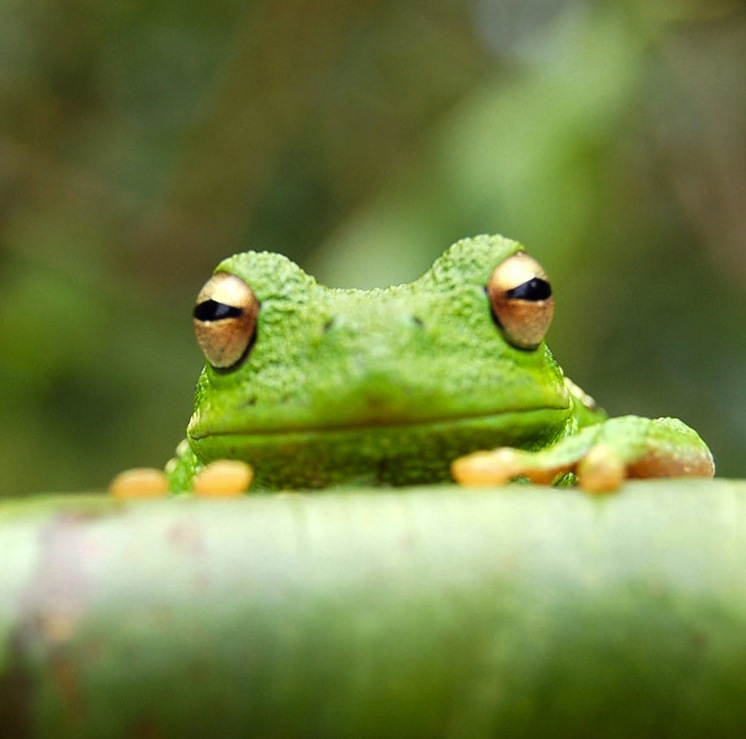
\includegraphics[width=0.3\textwidth]{frog.jpg}
\caption{\label{fig:frog}This frog was uploaded to writeLaTeX via the project menu.}
\end{figure}

\subsection{How to Make Tables}

Use the table and tabular commands for basic tables --- see Table~\ref{tab:widgets}, for example.

\begin{table}
\centering
\begin{tabular}{l|r}
Item & Quantity \\\hline
Widgets & 42 \\
Gadgets & 13
\end{tabular}
\caption{\label{tab:widgets}An example table.}
\end{table}

\subsection{How to Write Mathematics}

\LaTeX{} is great at typesetting mathematics. Let $X_1, X_2, \ldots, X_n$ be a sequence of independent and identically distributed random variables with $\text{E}[X_i] = \mu$ and $\text{Var}[X_i] = \sigma^2 < \infty$, and let
$$S_n = \frac{X_1 + X_2 + \cdots + X_n}{n}
      = \frac{1}{n}\sum_{i}^{n} X_i$$
denote their mean. Then as $n$ approaches infinity, the random variables $\sqrt{n}(S_n - \mu)$ converge in distribution to a normal $\mathcal{N}(0, \sigma^2)$.

\subsection{How to Make Sections and Subsections}

Use section and subsection commands to organize your document. \LaTeX{} handles all the formatting and numbering automatically. Use ref and label commands for cross-references.

\subsection{How to Make Lists}

You can make lists with automatic numbering \dots

\begin{enumerate}
\item Like this,
\item and like this.
\end{enumerate}
\dots or bullet points \dots
\begin{itemize}
\item Like this,
\item and like this.
\end{itemize}
\dots or with words and descriptions \dots
\begin{description}
\item[Word] Definition
\item[Concept] Explanation
\item[Idea] Text
\end{description}

We hope you find write\LaTeX\ useful, and please let us know if you have any feedback using the help menu above.
\end{comment}


\begin{thebibliography}{9}

\bibitem{code}
Code for Whatsup project. \url{https://github.com/samanca/whatsup}


\bibitem{network_tuning}
How to: network tuning. \url{http://wwwx.cs.unc.edu/~sparkst/howto/network_tuning.php}

\bibitem{youtube}
YouTube Architecture. \url{http://highscalability.com/youtube-architecture}

\bibitem{twitter}
Scaling Twitter: Making Twitter 10000 Percent Faster. \url{http://highscalability.com/scaling-twitter-making-twitter-10000-percent-faster}

%% whatsapp related
\bibitem{w1}
  WhatsApp. \url{http://www.whatsapp.com/}
  
\bibitem{w2}
  WhatsApp blog- Facebook. \url{http://blog.whatsapp.com/499/Facebook}
  
\bibitem{w3}
  Why Facebook needed WhatsApp. \url{http://www.theverge.com/2014/2/19/5428022/connect-or-die-why-facebook-needed-whatsapp}
  
\bibitem{w4}
The WhatsApp Architecture Facebook Bought For \$19 Billion. \url{http://highscalability.com/blog/2014/2/26/the-whatsapp-architecture-facebook-bought-for-19-billion.html}
  
  
%%erlang related  
\bibitem{erl_eprof}
  Erlang - eprof. \url{http://www.erlang.org/doc/man/eprof.html}
  
\bibitem{erl_fprof}
  Erlang - fprof. \url{http://www.erlang.org/doc/man/fprof.html}
  
%%ec2 related 
\bibitem{ec2_1}
  Amazon EC2 instances. \url{http://aws.amazon.com/ec2/instance-types/}

\bibitem{ec2_2}
	AWS Elastic Load Balancing. \url{http://aws.amazon.com/elasticloadbalancing/}
    
\bibitem{ec2_3}
Feature Guide: Amazon EC2 Elastic IP Addresses. \url{https://aws.amazon.com/articles/1346} 
%%server related

\bibitem{xmpp}
 XMPP. \url{http://xmpp.org/}
 
 \bibitem{smack}
 Ignite Realtime: Smack API. \url{www.igniterealtime.org/projects/smack}
  
\bibitem{ejabberd}
	ejabberd. \url{www.ejabberd.com}
    
 \bibitem{plugin_monitoring}
 	Monitoring plugin Readme. \url{http://www.igniterealtime.org/projects/openfire/plugins/monitoring/readme.html}
  
\bibitem{pubsub}
	Publish-subscribe pattern. \url{http://en.wikipedia.org/wiki/Publish\%E2\%80\%93subscribe_pattern}
    
\bibitem{bosh}
	BOSH. \url{www.xmpp.org/extensions/xep-0124.html}

\bibitem{openfire}
	Ignite Realtime- Openfire server \url{www.igniterealtime.org/projects/openfire/}
%%%
   
\bibitem{hazelcast}
	\url{http://www.igniterealtime.org/projects/openfire/plugins/hazelcast/readme.html}
    
\bibitem{mnesia}
mnesia. \url{http://www.erlang.org/doc/man/mnesia.html}

%%%tools
\bibitem{tools_munin}
  Munin - network resource monitoring tool. \url{www.munin.com}
  
\bibitem{tools_amazonc}
  AWS CloudWatch - Cloud \& Network Monitoring Services. \url{http://aws.amazon.com/cloudwatch/}
  
\bibitem{tools_amazond}
  Enabling or disabling detailed monitoring on EC2 instance. \url{http://docs.aws.amazon.com/AWSEC2/latest/UserGuide/using-cloudwatch-new.html}
  
\bibitem{tools_copper}
  CopperEgg. \url{http://copperegg.com/}
%%%%

\bibitem{erlang}
	Erlang Programming Language. \url{www.erlang.org}

\bibitem{tsung}
Tsung. \url{http://tsung.erlang-projects.org/}

\bibitem{ej1}
 ejabberd. \url{http://www.erlang.org/euc/04/jabber.pdf}

\bibitem{mongodb}
 {Plugge, Eelco and Hawkins, Tim and Membrey, Peter},
 {The Definitive Guide to MongoDB: The NoSQL Database for Cloud and Desktop Computing},
 {2010},
 {1430230517, 9781430230519},
 {1st},
 {Apress},
 {Berkely, CA, USA}.

\bibitem{instagram_ppt}
	Scaling instagram. \url{www.slideshare.net/iammutex/scaling-instagram}
    
\bibitem{slashdot}
	The Slashdot Effect, An Analysis of Three Internet Publications. \url{web.archive.org/web/20081202171653/http://ssadler.phy.bnl.gov/adler/SDE/SlashDotEffect.html}

%%%%%%

\end{thebibliography}


\section{Appendix}

\begin{figure*}[ht] \label{ fig7} 
  \begin{minipage}[b]{0.5\linewidth}
    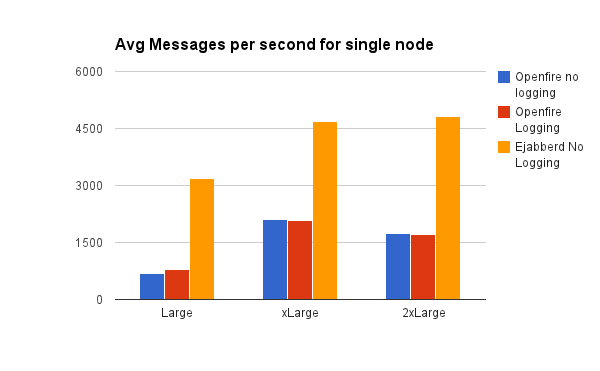
\includegraphics[width=0.9\linewidth]{image__12_.png} 
    \caption{Average messages per second for single node} 
  \end{minipage} 
  \begin{minipage}[b]{0.5\linewidth}
    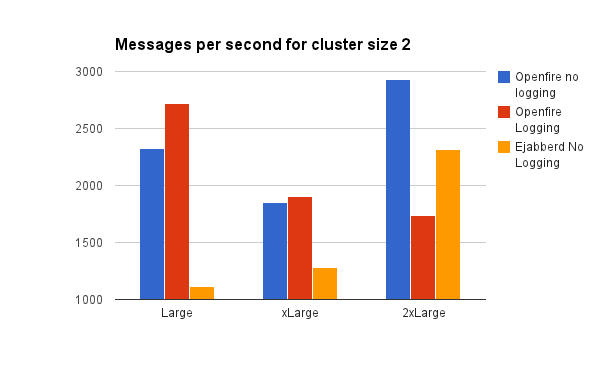
\includegraphics[width=0.9\linewidth]{image__13_.png} 
    \caption{Average messages per sec  for cluster 2} 
  \end{minipage} 
  \begin{minipage}[b]{0.5\linewidth}
    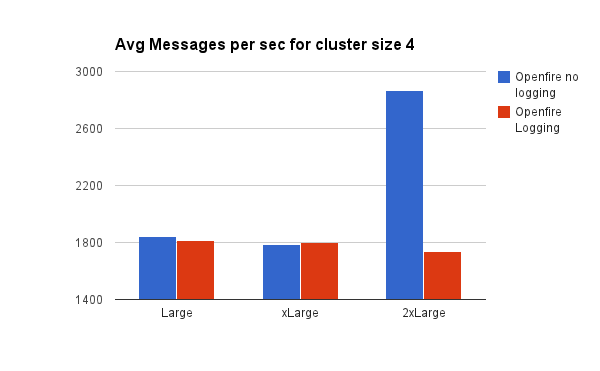
\includegraphics[width=0.9\linewidth]{image__14_.png} 
    \caption{Average messages per sec  for cluster 4} 
  \end{minipage}
  \hfill
  \begin{minipage}[b]{0.5\linewidth}
    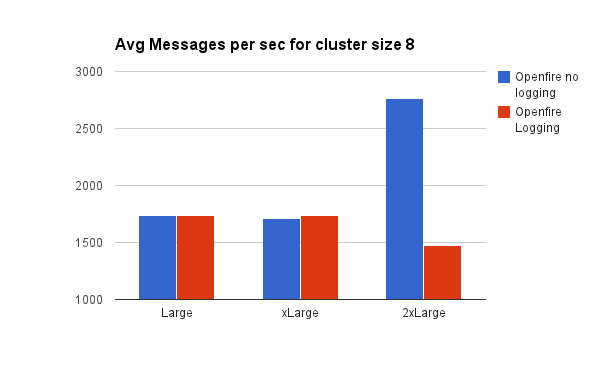
\includegraphics[width=0.9\linewidth]{image__15_.png} 
    \caption{Average messages per sec  for cluster 8} 
  \end{minipage} 
\end{figure*}

\begin{figure*}[ht] \label{ fig8} 
  \begin{minipage}[b]{0.5\linewidth}
    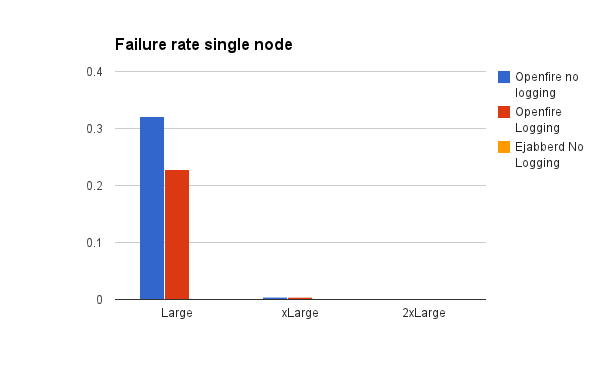
\includegraphics[width=0.9\linewidth]{image__16_.png} 
    \caption{Failure rate for single node} 
  \end{minipage} 
  \begin{minipage}[b]{0.5\linewidth}
    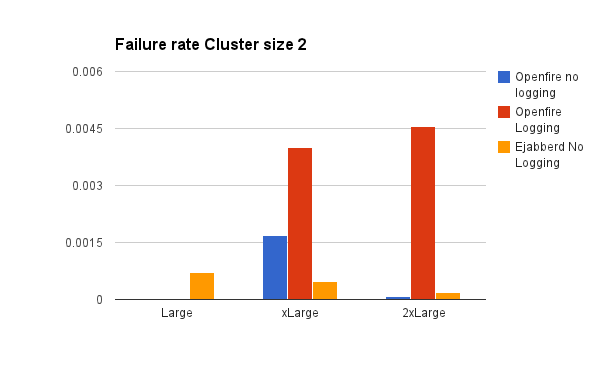
\includegraphics[width=0.9\linewidth]{image__17_.png} 
    \caption{Failure rate  for cluster 2} 
  \end{minipage} 
  \begin{minipage}[b]{0.5\linewidth}
    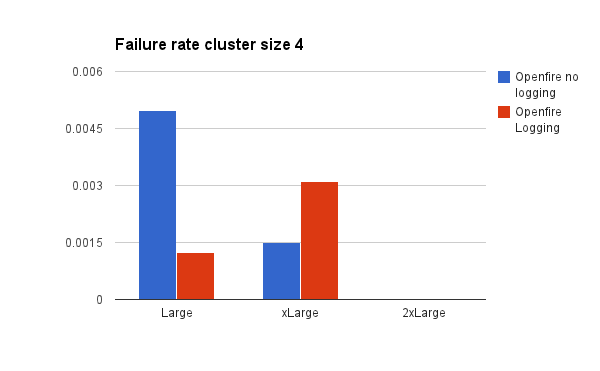
\includegraphics[width=0.9\linewidth]{image__18_.png} 
    \caption{Failure rate  for cluster 4} 
  \end{minipage}
  \hfill
  \begin{minipage}[b]{0.5\linewidth}
    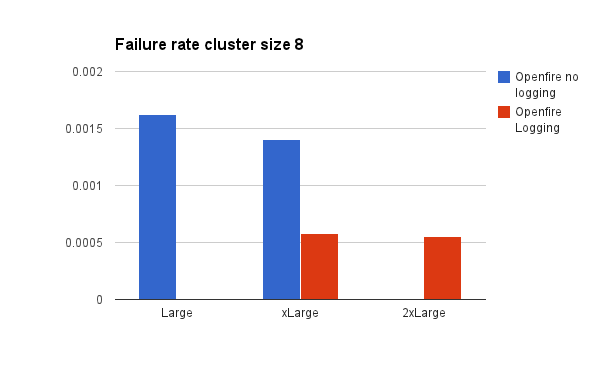
\includegraphics[width=0.9\linewidth]{image__19_.png} 
    \caption{Failure rate  for cluster 8} 
  \end{minipage} 
\end{figure*}

\begin{figure*}[ht] \label{ fig9} 
  \begin{minipage}[b]{0.5\linewidth}
    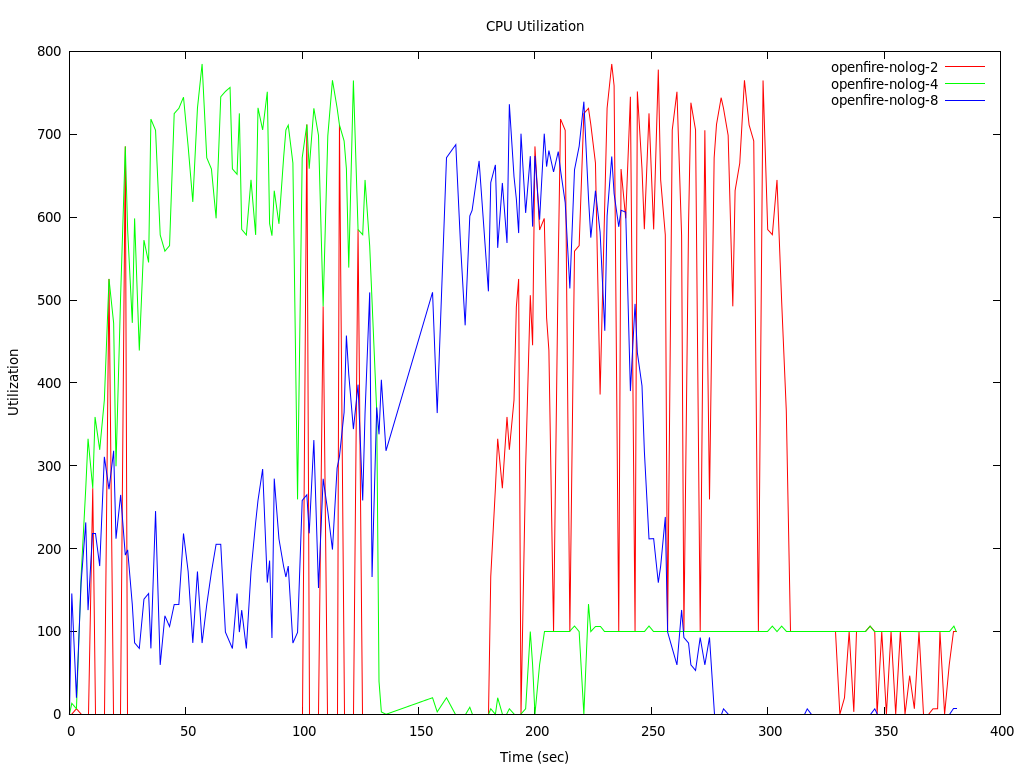
\includegraphics[width=0.9\linewidth]{2xlarge_cpu.png} 
    \caption{CPU Utilization for 2xLarge machines} 
  \end{minipage} 
  \begin{minipage}[b]{0.5\linewidth}
    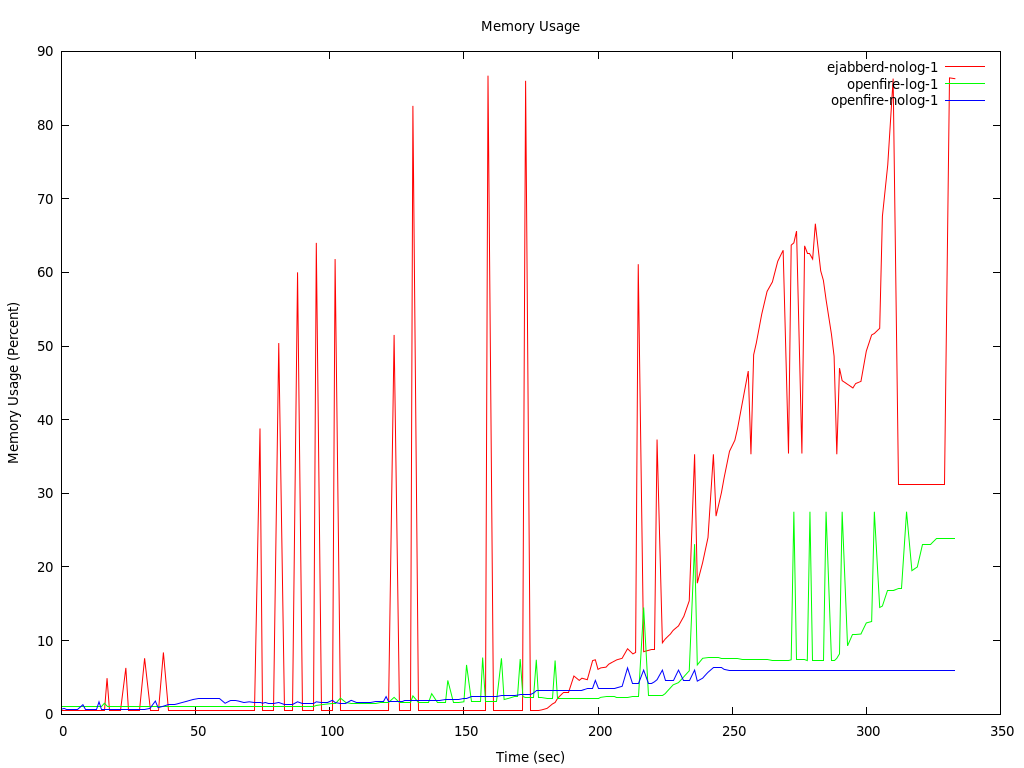
\includegraphics[width=0.9\linewidth]{2xlarge_memory.png} 
    \caption{Memory Usage for 2xLarge machines} 
  \end{minipage} 
\end{figure*}

\end{document}